\chapter{基于通道交换机制的跨模态RGB-D语义分割网络}
%此处主要是与上一章节的逻辑联系。要写一页。
语义分割是计算机视觉领域的一个重要研究任务,该任务旨在对给定图像的每一个像素进行分类。
在地铁排爆场景中,语义分割可以帮助机器人在复杂的场景下理解周边场景,进行定位、导航、排爆等任务。

近年来,卷积神经网络(Convolutional Neural Network,CNN)在高分辨率图像处理方面展示了强大的能力。
其中,全卷积网络(Fully Convolutional Network,FCN)是卷积神经网络在语义分割任务的重量级工作。
语义分割在彩色数据集上的迅速发展,随着RGB-D相机的发展,使用RGB-D数据的语义分割任务发展也如火如荼。

彩色数据和深度数据是同质化的图像信息,但是仍然是分属不同模态的数据,其中蕴含着的信息既有本模态的独特性,又有不同模态的互补性。

针对提取模态信息独特性而言,在传统的卷积操作中,卷积操作是为彩色信息设计的,并且在网络的训练过程中会和深度信息共享卷积参数,这样并不利于提取深度信息。

针对提取模态信息互补性而言,如何融合这种互补性信息,继而增强语义分割在RGB-D数据上的性能,是RGB-D语义分割领域的重中之重。
融合策略分为以下三种:前融合、中间融合、决策融合。
前融合就是指在输入进网络时,将彩色信息和深度信息做一个拼接操作,一起输入语义分割的网络之中。
中间融合就是在进行网络生成特征图之后,对生成的特征图使用融合策略,从而加强语义分割网络对特征的提取能力。
决策融合就是在网络进行最终分割结果运算时,将彩色信息的预测结果和深度信息的预测结果进行加强,得到最终的语义分割结构。
这三种融合策略并不是互相排斥的,他们可以共存在同一个分割网络之中。
由于前融合和决策融合较为简单,因此目前的研究重点主要是在中间层融合。

针对以上两个问题,本章首先提出了一种针对RGB-D双模态信息的卷积模块,该模块可以替换传统的卷积操作,应用在RGB-D语义分割网络中。其次,采用三种融合策略,构建一种基于特征图交换机制的中间融合机制,以加强RGB-D语义分割的性能。
具体而言,本章的主要工作包括几个部分:

(1)针对使用RGB-D双模态信息的语义分割网络,设计了一个跨模态卷积(Cross-modal convolution,CMConv),该部分可以更好地提取RGB-D信息,促进分割性能的提升。

(2)针对使用视觉transformer(vision transformer,VIT)的结构,
提出一种特征交换机制(Feature exchange),该结构可以有效地检测并剔除训练过程中的冗余特征信息,从而增强RGB-D语义分割网络的性能。





\section{模型方法}



\subsection{框架结构}



\subsection{跨模态卷积}
彩色信息和深度信息属于不同模态的信息。彩色图片通过对使用RGB色彩空间对颜色进行三通道赋值来表示捕获到的信息,而深度图片通过对捕获到的深度信息进行赋值产生的单通道灰白图片来表示捕获到的信息。因此,从本质上说,这两种数据是不同的。

从其表示信息的原理上来说,RGB值捕获投影图像空间中的光度外观属性,而深度特征编码局部形状信息及其在上下文中的位置信息。
对于同样形状的物体,我们希望网络可以提取出相同的特征。然而使用普通的卷积运算时,由于其位置的不同,提取出的特征是不同的,这阻碍了形状不变性的学习。
但是,也不能因为追求当前层的形状不变性而简单地将位置信息直接舍弃,因为位置信息在具有更大上下文的后续处理过程中会形成形状信息。
与位置相比,形状是物体更固有的属性,与语义联系更为紧密,因而对分割精度更关键。
因此,广泛用于使用彩色数据的卷积运算在处理深度数据时,并不高效。


基于深度特征可以表征形状信息和位置信息的模态特性,本章引入跨模态卷积来处理深度特征,以学习形状信息和位置信息重要性之间的自适应平衡,使网络有机会在必要时更多地关注形状信息,从而有利于RGB-D语义分割任务。

首先,将深度图片产生的补丁(patch)蕴含的形状信息和位置信息分解为两个独立的部分,得到形状分量(shape component)和位置分量(local component)。
深度补丁的平均值描述了该补丁在更大范围内的位置,从而构成了位置分量,表示距离观测点的距离。
而剩余的部分描述补丁的相对变化,描述了底层的几何形状,从而构成了形状分量,表示物体的语义。

然后,引入两个可学习的权值分别处理形状分量和位置分量得到形状核(shape kernal)和位置核(local kernal),最后对形状核和位置核加权组合,形成一个形状感知的补丁,并进一步与一个正常的卷积核进行卷积。
与原始补丁相比,形状感知补丁能够利用形状核自适应学习形状特征,利用位置核平衡形状和位置对最终预测的贡献。
此外,由于形状核和位置核在推理阶段成为常量,将它们融合到下面的卷积核中可以得到一个与普通卷积层相同的网络。


对于一个输入的补丁$\mathbb{P} \in R^{K_h \times K_w \times C_{in}}$,$K_h$和$K_w$是核的空间维度,$C_{in}$表示输入特征映射中的通道数,传统卷积层得到的输出特征
\begin{equation}
	\label{eq:conv}
	\mathbb{F} = Conv(\mathbb{K}, \mathbb{P}),
\end{equation}
其中,$\mathbb{K} \in R^{K_h \times K_w \times C_{in} \times C_{out}}$表示卷积层中核的可学习权值,$C_{out}$表示输出特征映射中的通道数。
$\mathbb{F} \in R^{C_{out}}$的每个元素计算为:
\begin{equation*}
	\mathbb{F}_{c_{out}} = \sum_{i}^{K_h \times K_w \times C_{in}} (\mathbb{K}_{i,c_{out}} \times \mathbb{P}_i).
	\label{eq:conv-f}
\end{equation*}

可以很容易地看出,$\mathbb{F}$通常会随着$\mathbb{P}$的不同值而变化。
假设有两个一样的物体在不同的位置,分别用补丁$\mathbb{P}_1$和补丁$\mathbb{P}_2$表示。
对应的输出特征:$\mathbb{F}_1$ and $\mathbb{F}_2$从卷积层学习:$\mathbb{F}_1 = Conv(\mathbb{K}, \mathbb{P}_1)$, $\mathbb{F}_2 = Conv(\mathbb{K}, \mathbb{P}_2)$。
由于$\mathbb{P}_1$和$\mathbb{P}_2$与观测点的距离并不相同,因此它们的特征通常不同,这可能导致不同的预测结果。
然而实际上,$\mathbb{P}_1$和$\mathbb{P}_2$属于同一个类别,传统的卷积层不能很好地处理这种情况。

但是,这两个补丁的形状是不变量。形状特征用来表征局部特征下的相对深度差异,而这一点却被现有的方法所忽略。
鉴于此,我们建议通过对RGB-D语义分割的形状进行有效建模来填补这一空白。

基于上述分析,本文提出将输入补丁分解为两个分量:描述补丁位置的位置分量(local component)和表示补丁是什么的形状分量(shape component)。

我们将补丁的平均值称为$\mathbb{P}_B$,其相对值称为$\mathbb{P}_S$。
\begin{equation*}
	\begin{aligned}
		& \mathbb{P}_B = m(\mathbb{P}), \\
		& \mathbb{P}_S = \mathbb{P} - m(\mathbb{P}),
	\end{aligned}
\end{equation*}
其中$m(\mathbb{P})$是$\mathbb{P}$ 上的平均函数(在$K_h \times K_w$维上),
$\mathbb{P}_B \in R^{1 \times 1 \times C_{in}}$,$\mathbb{P}_S \in R^{K_h \times K_w \times C_{in}}$。


注意,在等式\ref{eq:conv}中直接卷积的$\mathbb{P}_S$ with $\mathbb{K}$是次优的,因为来自$\mathbb{P}_B$的值有助于跨块的类别区分。
因此,我们的ShapeConv利用两个可学习的权重 $\mathbb{W}_B \in R^{1}$ and $\mathbb{W}_S \in R^{K_h \times K_w \times K_h \times K_w \times C_{in}}$来分别消耗上述两个分量。
然后以逐元素添加的方式组合输出的特征,这形成具有与原始$\mathbb{P}$相同大小的新的形状感知贴片。

\begin{equation}
	\label{eq:shapeconv-patch}
	\begin{aligned}
		\mathbb{F} &= ShapeConv(\mathbb{K}, \mathbb{W}_B, \mathbb{W}_S, \mathbb{P})\\
		&= Conv(\mathbb{K}, \mathbb{W}_B \diamond \mathbb{P}_B + \mathbb{W}_S \ast \mathbb{P}_S)\\
		&= Conv(\mathbb{K}, \textbf{P}_\textbf{B} + \textbf{P}_\textbf{S})\\
		&= Conv((\mathbb{K}, \textbf{P}_\textbf{BS}),
	\end{aligned}
\end{equation}
其中,$\diamond$ and $\ast$分别表示基本乘积和形状乘积算子,其被定义为

\begin{equation}
	\begin{cases}
		\textbf{P}_\textbf{B} = \mathbb{W}_B \diamond \mathbb{P}_B \\
		\textbf{P}_{\textbf{B}_{1,1,c_{in}}} = \mathbb{W}_B \times \mathbb{P}_{B_{1,1,c_{in}}},
	\end{cases}
	\label{eq:base-product-P}
\end{equation}
\begin{equation}
	\begin{cases}
		\textbf{P}_\textbf{S} = \mathbb{W}_S \ast \mathbb{P}_S \\
		\textbf{P}_{\textbf{S}_{{k_h},{k_w},{c_{in}}}} = \sum_{i}^{K_h \times K_w} (\mathbb{W}_{S_{i,{k_h},{k_w},{c_{in}}}} \times \mathbb{P}_{S_{i,{c_{in}}}}),
	\end{cases}
	\label{eq:shape-product-P}
\end{equation}

其中$c_{in}$, $k_h$, $k_w$分别是$C_{in}$, $K_h$, $K_w$维度中的元素的索引。

我们通过$\textbf{P}_\textbf{B}$ and $\textbf{P}_\textbf{S}$的相加来重建形状感知补丁$\textbf{P}_\textbf{BS}$,$\textbf{P}_\textbf{B}$ and $\textbf{P}_\textbf{S}$,这使得它能够被香草卷积层的内核$\mathbb{K}$平滑卷积。
然而,$\textbf{P}_\textbf{BS}$配备了通过两个额外权重学习的重要形状信息,使得卷积层专注于仅使用深度值失败的情况。

第3.1节中提出的形状转换可以有效地利用补丁。
然而,在CNNs中用ShapeConv代替香草卷积层引入了更多的计算成本,这是由于等式3和4中的两个乘积运算。为了解决这个问题,我们提出将这两个操作从补丁转移到内核
\begin{equation*}
	\begin{aligned}
		\begin{cases}
			\textbf{K}_\textbf{B} = \mathbb{W}_B \diamond \mathbb{K}_B \\
			\textbf{K}_{\textbf{B}_{1,1,c_{in},c_{out}}} = \mathbb{W}_B \times \mathbb{K}_{B_{1,1,c_{in},c_{out}}},
		\end{cases}
		\label{eq:base-product-K}
	\end{aligned}
\end{equation*}
\begin{equation*}
	\begin{aligned}
		\begin{cases}
			\textbf{K}_\textbf{S} = \mathbb{W}_S \ast \mathbb{K}_S \\
			\textbf{K}_{\textbf{S}_{{k_h},{k_w},{c_{in}},{c_{out}}}} = \sum_{i}^{K_h \times K_w} (\mathbb{W}_{S_{i,{k_h},{k_w},{c_{in}}}} \times \mathbb{K}_{S_{i,{c_{in}},{c_{out}}}}),
		\end{cases}
		\label{eq:shape-product-K}
	\end{aligned}
\end{equation*}

其中$\mathbb{K}_B \in R^{1 \times 1 \times C_{in} \times C_{out}}$ and $\mathbb{K}_S \in R^{K_h \times K_w \times C_{in} \times C_{out}}$分别表示核的基分量和形状分量,$\mathbb{K} = \mathbb{K}_B + \mathbb{K}_S$。因此,我们将方程2的形状转换重新形式化为以下:
\begin{equation}
	\label{eq:shapeconv-kernel}
	\begin{aligned}
		\mathbb{F} &= ShapeConv(\mathbb{K}, \mathbb{W}_B, \mathbb{W}_S, \mathbb{P})\\
		&= Conv(\mathbb{W}_B \diamond m(\mathbb{K})+ \mathbb{W}_S \ast (\mathbb{K} - m(\mathbb{K})), \mathbb{P})\\
		&= Conv(\mathbb{W}_B \diamond \mathbb{K}_B+ \mathbb{W}_S \ast \mathbb{K}_S, \mathbb{P})\\
		&= Conv(\textbf{K}_\textbf{B} + \textbf{K}_\textbf{S}, \mathbb{P})\\
		&= Conv(\textbf{K}_\textbf{BS}, \mathbb{P}),
	\end{aligned}
\end{equation}

其中 $m(\mathbb{K})$是$\mathbb{K}$上的平均函数(在$K_h \times K_w$维度上)。
我们要求$\textbf{K}_\textbf{BS} = \textbf{K}_\textbf{B} + \textbf{K}_\textbf{S}$, $\textbf{K}_\textbf{BS} \in R^{K_h \times K_w \times C_{in} \times C_{out}}$。

事实上,ShpeConv的两个公式,即,等式\ref{eq:shapeconv-patch}和等式\ref{eq:shapeconv-kernel}在数学上是等价的,即,
\begin{equation}
	\begin{aligned}
		\mathbb{F} &= ShapeConv(\mathbb{K}, \mathbb{W}_B, \mathbb{W}_S, \mathbb{P})\\
		&= Conv(\mathbb{K}, \textbf{P}_\textbf{BS})\\
		&= Conv(\textbf{K}_\textbf{BS}, \mathbb{P}),
	\end{aligned}
\end{equation}

\begin{equation}
	\begin{aligned}
		\mathbb{F}_{c_{out}} &= \sum_{i}^{K_h \times K_w \times C_{in}} (\mathbb{K}_{i,{c_{out}}} \times \textbf{P}_{\textbf{BS}_{i}})\\
		&= \sum_{i}^{K_h \times K_w \times C_{in}} (\textbf{K}_{\textbf{BS}_{i,{c_{out}}}} \times \mathbb{P}_{i}),
	\end{aligned}
\end{equation}


推论阶段。在推理过程中,由于$\mathbb{W}_B$ and $\mathbb{W}_S$这两个附加权重变为常数,因此我们可以将它们融合成$\textbf{K}_\textbf{BS}$,如\ref{fig:ShapeConv}(c)所示$\textbf{K}_\textbf{BS} = \mathbb{W}_B \diamond \mathbb{K}_B+ \mathbb{W}_S \ast \mathbb{K}_S$。
$\textbf{K}_\textbf{BS}$与等式\ref{eq:conv}中的$\mathbb{K}$共享相同的张量大小,因此,我们的ShapeConv实际上与\ref{fig:ShapeConv}(a)中的香草卷积层相同。换句话说,当用ShapeConv代替香草卷积时,不会引入额外的推理时间。


%\subsection{特征交换机制}
如引言中所讨论的,深度多模态融合方法主要可以分为基于聚合的融合和基于融合的融合[4]。
由于模态内处理的弱点,最近的基于聚合的工作执行特征融合,同时仍然保持所有模态的子网络[12,30]。
此外,[19]指出,熔合的性能受到选择熔合哪一层的高度影响。
基于对齐的融合方法通过应用相似性规则来对齐多模态特征,其中最大均值差异MMD)[16]通常用于测量。
然而,仅仅关注统一整个分布可能会忽略每个领域/模态中的特定模式[6,44]。
因此,[47]提供了一种可以缓解这一问题的方法,该方法将模态共同特征相关联,同时保持模态特定信息。
还有一部分基于调制的多模态学习文献[11,13,46]。
不同于这些类型的融合方法,我们提出了一种新的融合方法,通过通道交换,这可能享有充分的模型间的相互作用和模态内学习的保证。
使用BN缩放因子来评估CNN通道重要性的想法已经在网络修剪[33,49]和表示学习[40]中进行了研究。
[33]对缩放因子实施了101范数惩罚,并显式地修剪掉满足稀疏性标准的过滤器。
在这里,我们将这个想法作为一种自适应工具来确定在哪里交换和融合。
CBN [46]通过以另一种模态为条件调制一种模态的BN来执行跨模态消息传递,这显然不同于我们在不同模态之间直接交换信道以进行融合的方法。
ShuffleNet [53]提出在多个组之间移动一部分信道,以在轻量级网络中进行有效传播,这类似于我们交换信道进行消息融合的想法。
然而,虽然我们的论文的动机是非常不同的,但交换过程是由BN缩放因子自决定的,而不是ShuffleNet中的随机交换。








Transformer最初在自然语言社区中被广泛研究为非递归序列模型[40],并且很快被扩展以使视觉语言任务受益。最近,许多研究进一步采用变压器进行计算机视觉任务,具有良好的适应性架构和优化时间表。因此,视觉跨以前的变体已经在许多单模视觉任务中显示出巨大的潜力,例如分类[6,21]、分割[44,47]、检测[3,8,22,48]、图像生成[16]。然而,直到这项工作的日期,尝试扩展视觉转换器,以处理多模态数据仍然很少。当引入具有复杂对齐关系的多模态数据时,对模型体系结构的融合方案设计提出了很大的挑战。要回答的关键问题是,不同模态的特征之间的交互应如何以及在何处发生。已有几种基于变换器的视觉语言融合方法,VL-BERT [37]和ViLT [17]中所述的方法。在这些方法中,视觉和语言标记在每个Transformer层之前直接级联,使得整体架构与原始Transformer非常相似。这种融合通常是比对不可知的,这表明没有明确地利用模态间比对。我们还尝试将类似的融合方法应用于多模态视觉任务(第4)、第四章。不幸的是,这种直观的Transformer融合不能带来有希望的增益,或者甚至可能导致比单模态对应物更差的性能,这主要是由于没有充分利用模态间的相互作用。也有几种尝试用于融合多种视觉模态。例如,TransFuser [26]利用Transformer模块来连接图像的CNN主干和LiDAR点。与已有的试验不同,本文旨在寻求一种有效且通用的方法,将多个单模态变压器组合起来,并在模型中插入模态间的对齐。这项工作有利于多模态数据的学习过程,同时利用模态间对齐。这种对准在许多视觉任务中自然可用,例如,利用摄像机内函数/外函数,世界空间点可以被投影并且对应于摄像机平面上的像素。与不可知论融合(Sec.3.1),该martaware融合明确涉及的对齐关系,
不同的模式。然而,由于在Transformer中引入了模态间投影,因此对准感知融合可能会极大地改变原始模型结构和数据流,这可能会破坏单模态架构设计的成功或预训练期间习得的注意力。因此,可能必须为多模投影和融合确定“正确的”层/记号/通道,并且还必须为新模型重新设计架构或重新调整优化设置。为了避免处理这些具有挑战性的问题并继承原始单模设计的大部分,我们提出了多模式令牌融合,称为TokenFusion,它自适应地并有效地融合多个单模变换器。我们的TokenFusion的基本思想是修剪多个单模态变换器,然后重新利用修剪后的单元进行多模态融合。我们对每个单模态Transformer应用单独的修剪,并且每个修剪的单元由来自其他模态的投影对准特征代替。假设该融合方案对原始的单模态变压器具有有限的影响,因为它保持了重要单元的相对注意关系。TokenFusion在允许多模态转换器继承来自单模态预训练的参数方面也被证明是上级的,在ImageNet上。展示优势


融合视觉变形。与多模态数据的深度融合一直是一个重要的主题,它可能通过利用多个输入源来提高性能,并且还可能进一步释放变压器的力量。然而,将多个现成的单变压器联合收割机组合在一起,同时保证这种组合不会影响其精心设计的单模态设计,这是具有挑战性的。信号装置.[2]以及[20]利用变换器处理连续的视频帧,用于空间-时间对准,并通过使多个帧相关来捕获细粒度模式。关于多模态数据,[26,41]利用Transformer模块的动态特性来联合收割机CNN主干,以融合红外/可见光图像或LiDAR点。[9]将从粗到精的经验从CNN融合方法扩展到用于图像处理任务的变换器。[14]采用变换器联合收割机高光谱图像进行简单的特征拼接。[24]在图像补片和音频频谱图补片之间插入中间标记作为瓶颈以隐式地学习模态间对准。然而,这些工作与我们的工作不同,因为我们希望构建一个通用的融合管道,用于组合现成的视觉转换器,而无需重新设计其结构或重新调整其优化设置,同时明确利用模态间的对齐关系。


Vision Transformers的基本融合

假设我们有第$i$个输入数据$\bm{x}^{(i)}$,它包含$M$个模态:$\bm{x}^{(i)}=\{\bm{x}_m^{(i)}\in\mathbb{R}^{N\times C}\}_{m=1}^M$,其中$N$ and $C$分别表示令牌和输入通道的数量。
为了简单起见,我们将在接下来的部分中省略下标$^{(i)}$。
深度多模态融合的目标是确定一个多层模型 $f(\bm{x})$,期望其输出尽可能接近目标$\bm{y}$。
具体来说,在这项工作中,$f(\bm{x})$是近似基于transformerbased网络架构。
假设模型总共包含$L$ 层,我们表示第$l$层($l=1,\ldots,L$)为$\bm{e}^l=\{\bm{e}^l_m\in\mathbb{R}^{N\times C'}\}_{m=1}^M$,其中$C'$表示范围内的层的特征通道的数量。最初,使用$\bm{e}_m^1$的线性投影来获得$\bm{x}_m$,这是一种广泛采用的对输入标记(例如,图像块)进行矢量化的方法,使得第一Transformer层可以接受标记作为输入。





我们对输入模态使用不同的变换器,并将$f_m(\bm{x})=\bm{e}_m^{L+1}$表示为第$m$个Transformer的最终预测。给定第$m$个模态的令牌特征$\bm{e}_m^{l}$,第$l$层计算





翻译到这里 懂?
1这是第三章节 懂?1
还有什么问题?我试试不动了喊你1
\subsection{Vision Transformer 的基本融合}
\label{subsec:intuitive_fusion}
假设我们有第$i$个输入数据$\bm{x}^{(i)}$它包含$M$个模态: $\bm{x}^{(i)}=\{\bm{x}_m^{(i)}\in\mathbb{R}^{N\times C}\}_{m=1}^M$,其中,$N$ 和$C$分别表示令牌和输入通道的数量。 
为了简单起见,我们将在接下来的部分中省略下标$^{(i)}$ 。
深度多模态融合的目标是确定一个多层模型 $f(\bm{x})$,期望其输出尽可能接近目标 $\bm{y}$ 。 
具体来说,在这项工作中,$f(\bm{x})$是近似基于transformerbased的网络架构。假设模型总共包含$L$层, 我们表示第$l$层($l=1,\ldots,L$)为$\bm{e}^l=\{\bm{e}^l_m\in\mathbb{R}^{N\times C'}\}_{m=1}^M$, 其中$C'$表示范围内的层的特征通道的数量。
最初,使用$\bm{x}_m$的线性投影来获得$\bm{e}_m^1$,这是一种广泛采用的对输入标记(\emph{例如},图像块)进行矢量化的方法,使得第一Transformer层可以接受标记作为输入。

我们对输入模态使用不同的变换器,并将$f_m(\bm{x})=\bm{e}_m^{L+1}$表示为第$m$个Transformer的最终预测。
给定第$m$个模态的令牌特征$\bm{e}_m^{l}$,第$l$层计算
\begin{equation}
	\label{eq:token-feature}
	\hat{\bm{e}}_m^l=\text{MSA}\big(\text{LN}(\bm{e}_m^{l})\big),\; \bm{e}_m^{l+1}=\text{MLP}\big(\text{LN}(\hat{\bm{e}}_m^l)\big),
\end{equation}
其中$\text{MSA}$, $\text{MLP}$,和 $\text{LN}$表示多头自注意、多层感知和层归一化,
$\hat{\bm{e}}^l_m$ 代表MSA的输出。 

在视觉任务的多模态融合过程中,不同模态的对齐关系可以显式地可用。例如,像素位置通常用于确定图像深度相关性;并且相机内函数/外函数在将3D点投影到图像中时很重要。基于对齐信息的参与,我们考虑了以下两种Transformer融合方法。

对齐不可知融合不明确使用模态之间的对齐关系。该算法期望从大量的数据中隐式地学习到对齐。对齐不可知融合的一种常用方法是直接拼接多模态输入标记,广泛应用于视觉语言模型。类似地,用于第$l$层的输入特征$\bm{e}_l$也是不同模态的令牌式级联。尽管对准不可知的融合是简单的并且可以对原始Transformer模型具有最小的修改,但是很难直接受益于已知的多模态对准关系。

\label{sec:对齐感知融合}明确地利用模态间对齐。例如,这可以通过选择对应于相同像素或3D坐标的标记来实现。假设$\bm{x}_m[n]$是第$m$个模态输入$\bm{x}_m$的第$n$个令牌,其中$n=1,\cdots,N_m$。我们将从第$m$个模态到第$m'$个模态的“标记投影”定义为:
\begin{equation}
	\label{eq:token-projection}
	\mathrm{Proj}^\text{T}_{m'}(\bm{x}_{m}[n_{m}])=h(\bm{x}_{m'}[n_{m'}]),
\end{equation}
其中$h$可以简单地是身份函数(对于同质模态)或浅多层感知(对于异质模态)。当考虑整个$N$个token时,我们可以方便地将“模态投影”定义为token投影的串联:
projections:\vskip-0.2in
\begin{equation}
	\label{eq:modality-projection}
	{\mathrm{Proj}}^\text{M}_{m'}(\bm{x}_{m})=\big[\mathrm{Proj}^\text{T}_{m'}(\bm{x}_{m}[1]); \cdots; \mathrm{Proj}^\text{T}_{m'}(\bm{x}_{m}[N])\big].
\end{equation}

\ref{eq:modality-projection} 仅示出了输入侧的融合策略。我们还可以通过投影和聚合特征嵌入$\bm{e}_m$,在不同模态特定模型之间执行中间层或多层融合,这可能实现更多样化和更精确的特征交互。
然而,随着基于变换器的模型的复杂性的增长,搜索仅用于两种模态 (\emph{例如} 2D和3D检测变换器)的最佳融合策略(\emph{例如} 应用投影和聚集的层和标记)可能会增长为极难解决的问题。 
为了解决这一问题, 我们在第2.3节中提出了多模式令牌融合 \ref{subsec:mix_transformers}.



\subsection{多模式令牌融合}
\label{subsec:mix_transformers}



正如 \ref{sec:intro}描述的, 多模态令牌融合 (TokenFusion) 首先修剪单模态变换器,并进一步重新利用修剪后的单元进行融合。通过这种方式,原始的单模态变压器的信息单元被假定为在很大程度上被保留,而多模态的相互作用可以被涉及以提高性能。

如之前在\cite{DBLP:journals/corr/abs-2106-02034}中所示,视觉变换器的标记可以在保持性能的同时以分层方式被修剪。类似地,我们可以通过采用评分函数$s^l(\bm{e}^{l})=\text{MLP}(\bm{e}^{l})\in[0,1]^N$来选择较少信息的标记, 该评分函数动态地预测第$l$层和第$m$模态的标记的重要性。
为了在$s^l(\bm{e}^{l})$上实现反向传播,我们重新公式化方程中的MSA输出$\hat{\bm{e}}_m^l$ in \ref{eq:token-feature} as 
\begin{equation}
	\label{eq:msa-output-score}
	\hat{\bm{e}}_m^l=\text{MSA}\big(\text{LN}(\bm{e}_m^{l})\cdot s^l(\bm{e}_m^{l})\big).
\end{equation}

我们使用$\mathcal{L}_m$来表示第$m$个模态的任务特定损失。为了修剪无信息的标记,我们进一步在$s^l(\bm{e}_m^{l})$上添加标记式修剪损失($l_1$-norm)。因此,用于优化的总损失函数被导出为:
\vskip-0.1in
\begin{equation}
	\label{eq:overall-loss}
	\mathcal{L}=\sum_{m=1}^M\Big(\mathcal{L}_m+\lambda\sum_{l=1}^L\big|s^l(\bm{e}_m^{l})\big|\Big),
\end{equation}
其中$\lambda$ 是用于平衡不同损耗的超参数。

对于特征$\bm{e}_m^l\in\mathbb{R}^{N\times C'}$,令牌式剪枝从所有$N$个令牌中动态检测不重要的令牌。改变不重要的标记或用其他嵌入替换它们,预计对其他信息标记的影响有限。
因此,我们提出了一种用于多模态变换器的标记融合过程,因此,我们为多模态变换器提出了一种标记融合程序,用其他模态的标记投影(定义见第 \ref{sec:alignment-aware-fusion}节)替代不重要的标记。
由于修剪过程是动态的,{\emph{i.e.}},即,在输入特征的条件下,融合过程也是动态的。该过程在每个Transformer层之前执行令牌替换,因此第$l$层的输入特征,\emph{i.e.},$\bm{e}_m^l$,被重新表述为\vskip-0.2in
\begin{align}
	\label{eq:mix-process}
	\bm{e}_m^l&=\bm{e}_m^l\odot\mathbb{I}_{s^l(\bm{e}_m^{l})\ge\theta}
	+{\mathrm{Proj}}^\text{M}_{m'}(\bm{e}_m^l)\odot\mathbb{I}_{s^l(\bm{e}_m^{l})<\theta},
\end{align}
其中$\mathbb{I}$是一个断言下标条件的指示符,因此它输出一个掩码张量$\in\{0,1\}^N$;参数$\theta$是一个小阈值(我们在实验中采用$10^{-2}$);运算符$\odot$ 表示逐元素乘法。

In \ref{eq:mix-process}, 如果只有两个模态作为输入,则$m'$将仅仅是除$m$之外的另一模态。对于两个以上的模态,我们将标记预先分配为$M-1$个部分,每个部分都与其他模态中的一个绑定,而不是与它绑定。此预分配的更多细节将在\ref{subsec:homogeneous-modalities}. 


\subsection{剩余位置对准} 
\label{subsec:rpa}
直接替换代币将冒着完全破坏其原始位置信息的风险。
因此,模型仍然可以忽略来自另一模态的投影特征的对齐。
为了缓解这个问题,我们采用了残余位置对齐(RPA),利用位置嵌入(PE)的多模式对齐。
图\ref{pic:framework} and 图\ref{pic:framework-hete} 所示。
稍后将详细介绍,RPA 的关键理念在于向后续层注入等效 PE。
此外,PE的反向传播在第一层之后停止,这意味着在整个训练过程中,仅保留第一层处的PE的梯度,而对于其余的层则冻结。以这种方式,PE服务于对齐多模态令牌的目的,而不管原始令牌的替换状态。总之,即使替换了标记,我们仍然保留从另一个模态添加到投影特征的原始PE。 



\begin{figure}[t!]
	\centering
	\hskip0.07in
	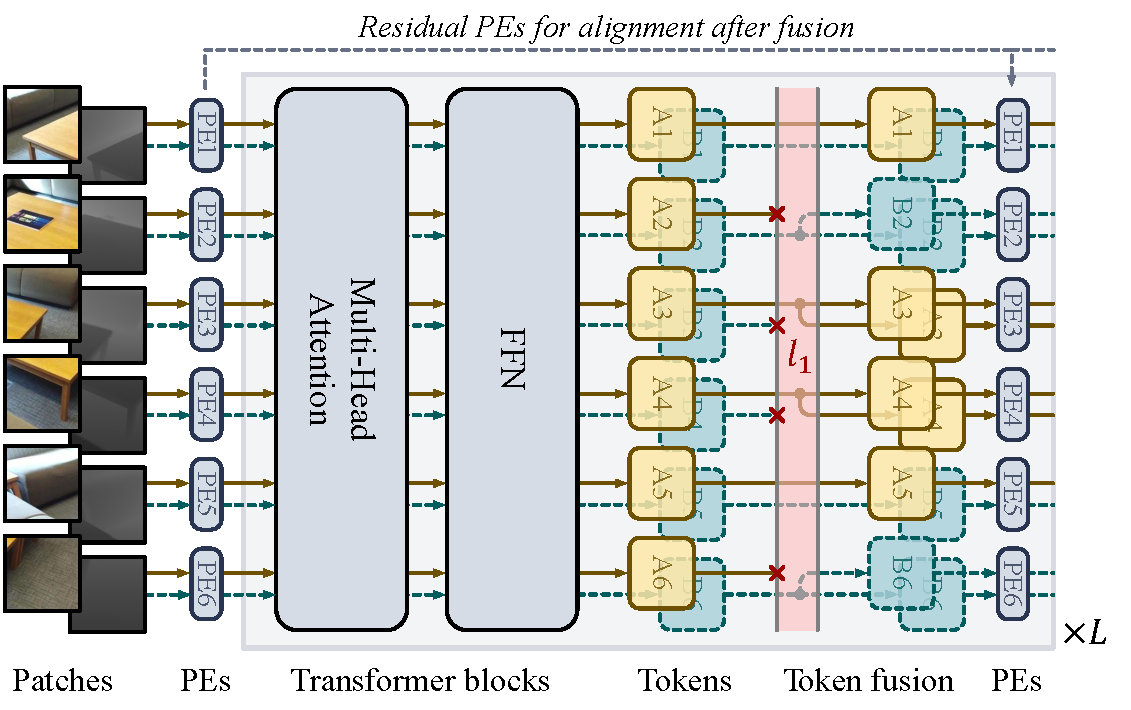
\includegraphics[scale=0.42]{figures/mixt-ho.pdf}
	\caption[]{以RGB和深度为例,介绍了一种用于同质模态的TokenFusion框架。这两种模态都被发送到共享的Transformer,其中还具有共享的位置嵌入。}
	\label{pic:framework}
	\vskip-0.1in
\end{figure}

\begin{figure*}[t!]
	\centering
	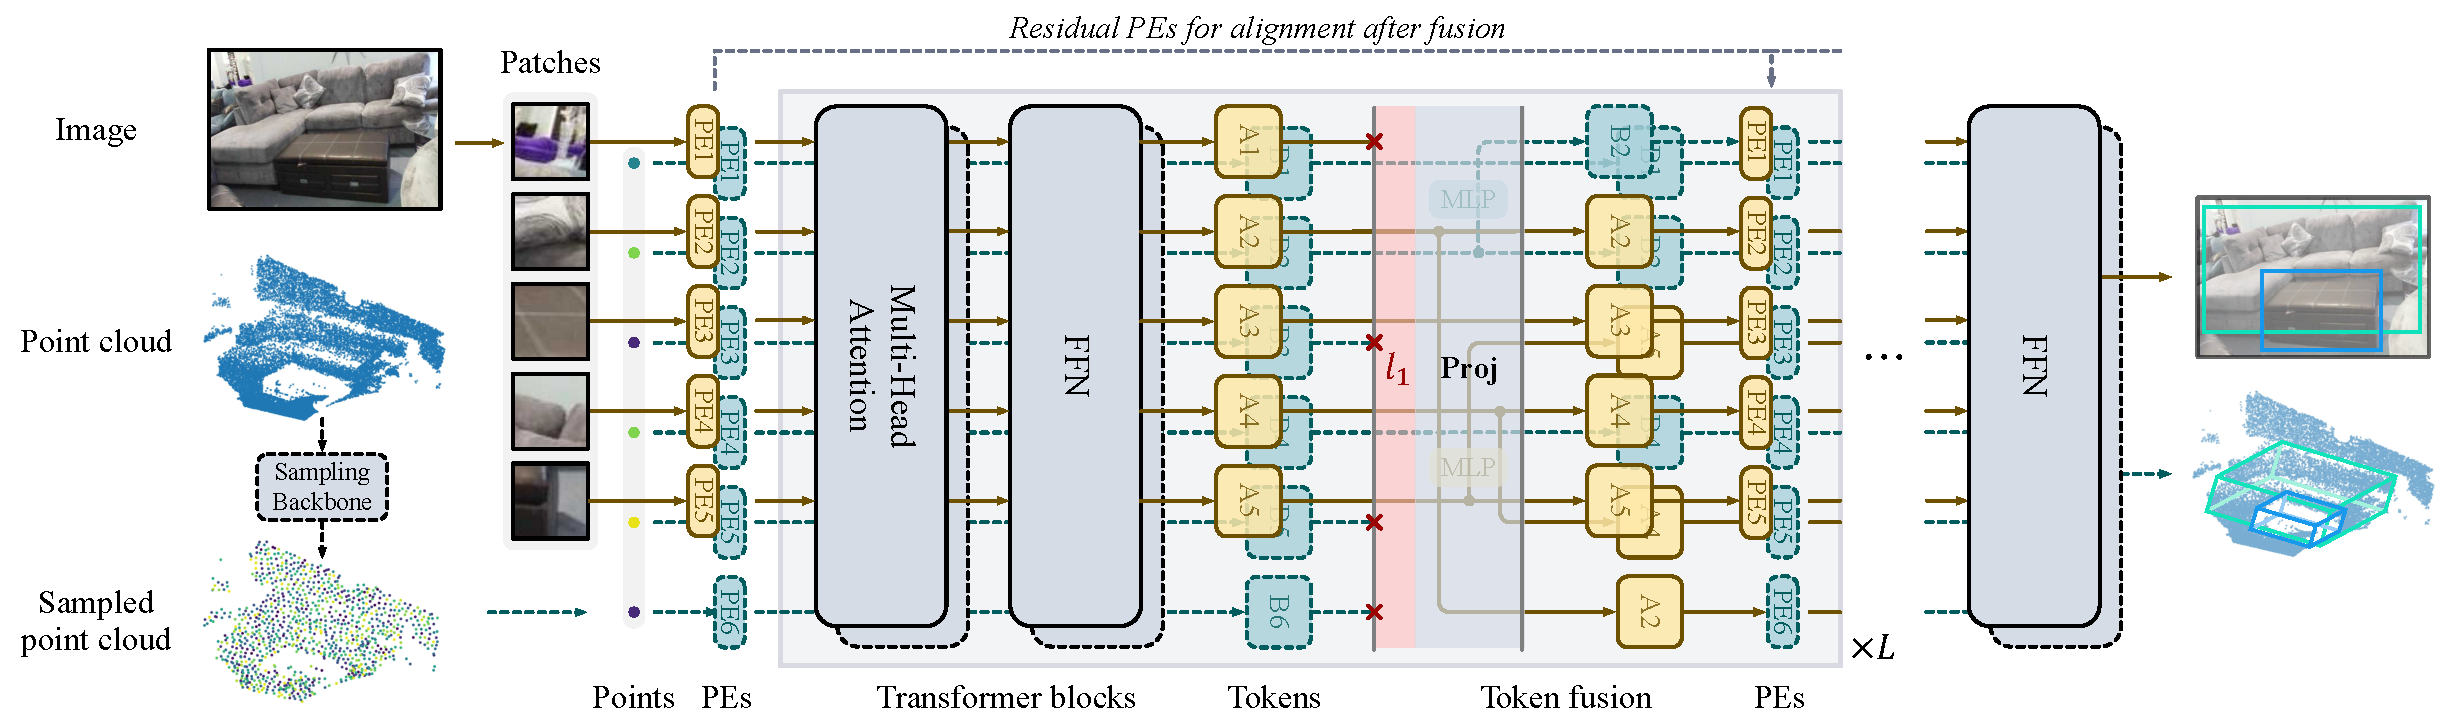
\includegraphics[scale=0.42]{figures/mixt-he.pdf}
	\caption[]{用于点云和图像的异构模态的TokenFusion框架。两种模态都被发送到具有单独位置嵌入的单独Transformer模块。需要额外的模态间投影(Proj),这与同质模态的融合不同
	}
	\label{pic:framework-hete}
	\vskip-0.1in
\end{figure*}




